\chapter{Resultat}

I detta kapitel redovisas det resulterande läromaterialet, vilket består av fem
kapitel. Det är publicerat på en hemsida och dess källkod är fritt tillgänglig.
Även resultaten från utvärderingen med testgruppen och mötena med Åke Fäldt
redovisas.

\section{Läromaterialet}\label{sec:res_laromaterial}

Detta avsnitt innehåller en översikt av läromaterialet samt ett axplock av innehållet ur
vardera kapitel. Axplocken exemplifier delar av läromaterialet och
implementationerna av de domänspecifika språken. De fullständiga implementationerna
är inte inkluderade (och förklarade) eftersom det är precis det läromaterialet
innehåller. Rapporten skulle då bli en kopia av läromaterialet. Istället finns hela läromaterialet i bilaga~\ref{cha:utdrag} samt hemsidan~\cite{LYAP} där det blev publicerat. De avsnitt i rapporten som beskriver läromaterialets innehåll är inga
exakta kopior ord-för-ord utan de har anpassats till
rapporten.

\subsection{Översikt}

Läromaterialet är en löpande text där Haskell-kod och lärotext sammanvävts. Det
ser ut som i figur~\ref{fig:smakprov_laromaterial}. Lärotexten förklarar både fysik, Haskell och hur de relaterar till varandra. I texten följer läsaren med
i implementationen av ett domänspecifikt språk och det visas hur det används.
Tanken är att läsaren parallellt programmerar det som texten förklarar, för att
på så sätt även få praktisk färdighet i det som presenterats. För detta syfte
finns det även övningar tillagda direkt i den löpande texten, se
figur~\ref{fig:smakprov_ovning}, som ofta innebär att läsaren själv ska
implementera en liten del av det domänspecifika språket. Det finns också
övningar i slutet av kapitlet som ofta innebär större vidareutvecklingar av de
domänspecifika språken.

\begin{figure}[h]
    \centering
    \begin{subfigure}[t]{0.5\textwidth}
        \centering
        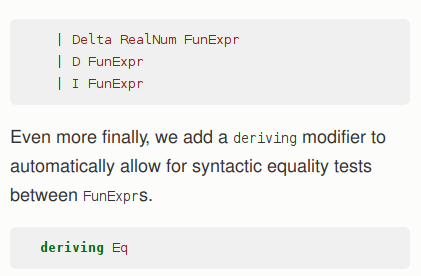
\includegraphics[width=0.9\linewidth]{figure/smakprov_laromaterial.png}
        \caption{Lärotexten är mot den ljusgrå bakgrunden medan Haskell-kod är mot den mörkgrå.}~\label{fig:smakprov_laromaterial}
    \end{subfigure}%
    ~~~
    \begin{subfigure}[t]{0.5\textwidth}
        \centering
        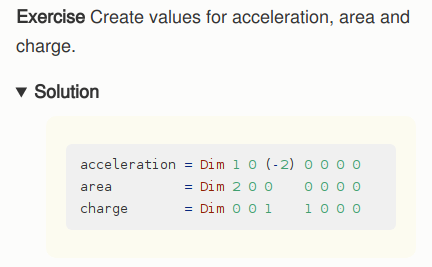
\includegraphics[width=0.9\linewidth]{figure/smakprov_ovning.png}
        \caption{Exempel på en övning. Övningen ligger som en del av den
                 löpande texten.}~\label{fig:smakprov_ovning}
    \end{subfigure}
    \caption{Ett smakprov av det resulterande läromaterialet.}
\end{figure}

Språket i lärotexten är enligt projektgruppen lättsamt\footnote{Diskuteras
utförligare i avsnitt \ref{sec:res_disk}.} och i detta syfte finns det även
bilder tillagda. Figur~\ref{fig:smakprov_bild_laromaterial} är ett exempel på en
bild ur läromaterialet. Notera speciellt den medvetet oseriösa ritningstekniken
som är tänkt att vara rolig och muntra upp läsaren.\newline

% newline ska kanske bort. Är för formatering

\begin{figure}[h]
        \centering
        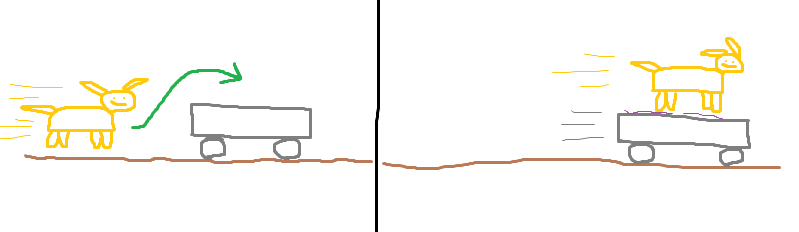
\includegraphics[width=0.4\linewidth]{figure/smakprov_bild_laromaterial.png}
        \caption{Exempel på en bild. Bilden visar hur en hund springer och hoppar upp på en stillastående vagn.}
        \label{fig:smakprov_bild_laromaterial}
\end{figure}

Läromaterialet innehåller fem kapitel som vardera behandlar ett område inom fysik
och matematik. Fokuset är på klassisk mekanik samt den matematik som tillhör
området. De behandlade områdena är:

\begin{itemize}
  \item Dimensioner
  \item Matematisk analys
  \item Vektorer
  \item Exempelproblem
  \item Partikelmekanik
\end{itemize}

\textit{Dimensioner} behandlar fysikaliska dimensioner, storheter och enheter inom fysiken.
Fysikaliska dimensioner införs på typnivå i Haskell för att visa likheten mellan
Haskells typsystem och hur dimensioner hanteras inom fysiken.
Typnivåprogrammering\footnote{Vanligtvis manipuleras \textit{värden} när
programmerering sker i Haskell och andra språk. Typnivåprogrammering är precis som
vanlig programmering med skillnaden att den sker på typnivån, det vill säga, att
typer modifieras. För en utförligare förklaring av typnivåprogrammering, se läromaterialet~\cite{LYAP}.} används för att göra likheterna så tydliga som möjligt.

I \textit{matematisk analys} behandlas differentialkalkyl och
integralkalkyl för en variabel. Först bestäms den semantiska domänen
för analys i en variabel: reella funktioner av ett argument; och ett syntaxträd
för uttryck av funktioner inom denna domän konstrueras. Därefter
analyseras syntax och semantik för differenser, derivator, och
integraler; och funktioner implementeras för att utföra dessa
operationer både approximativt numeriskt, och symboliskt med ett
syntaxträd. Slutligen appliceras de implementerade funktionerna för
att visualisera grafer av operationerna.

\textit{Vektorer} behandlar vektorer och vektoroperationer. Vektorer modelleras
med hjälp av en typklass som dikterar vilka funktioner som varje
modell av en vektor måste implementera. Generella vektoroperationer såsom
addition och skalärprodukt implementeras sedan med hjälp av dessa funktioner
vilket skapade ett mycket generellt och lättanvänt gränssnitt. QuickCheck
användes för att verifiera lagarna som gäller för olika vektoroperationer,
vilket gav en generell säkerhet kring att implementationerna var korrekta.

I \textit{exempelproblem} tillämpas de tre tidigare kapitlen på två vanliga
mekanikproblem, nämligen \textit{krafter på lådor} och \textit{gungbräda}. I
krafter på lådor används det domänspecifika språket för vektorer till att
beräkna de krafter som verkar på en låda som glider ner för ett plan. I
gungbräda visas hur momentjämviktsberäkningar kan göras med det domänspecifika
språket för dimensioner.

\textit{Partikelmekanik}. En repetition av gymnasieskolans fysik.
Lägesenergi, rörelseenergi, gravitation och så vidare. Den modelleras med vektorer vars
komponenter består av matematiska uttryck tagna från kapitlet om matematisk
analys. Förhoppningen är att detta område inte ska presentera någon ny fysik för
läsaren utan istället visa hur redan känd fysik direkt går att översätta till
läromaterialets domänspecifika språk.

Läromaterialet blev publicerat på en hemsida~\cite{LYAP} och all källkod finns
tillgänglig på projektets GitHub~\cite{LYAP_repo}. På GitHub finns även ett
antal delvis färdigställda områden, till exempel bevisföring. Texten i
läromaterialet är skriven på engelska.

\subsection{Dimensioner}
\label{sec:grund_impl}
\label{sec:res_dim}

I detta avsnitt visas delar av hur implementationen av dimensioner ser ut i
läromaterialet. Den fullständiga implementationen innehåller tre delar:

\begin{enumerate}
  \item Dimensioner på värdenivå
  \item Dimensioner på typnivå
  \item Datatyp för storheter
\end{enumerate}

Dimensioner på värdenivå används för att enkelt kunna skriva ut dimensioner i
GHCi. Dimensioner på typnivå används för att ge typsäkerhet till dimensioner, så
att till exempel en längd och en massa inte kan adderas, likt att ett värde av
typ \texttt{Double} och \texttt{Integer} inte kan adderas i Haskell. Till sist
kombineras de två varianterna av dimensioner till en datatyp för storheter som
aritmetiska operationer kan utföras på.

Dimensioner kan ses som en produkt av de 7 basdimensionerna\footnote{Längd,
massa, tid, elektrisk ström, temperatur, substansmängd och ljusstyrka.}, med en
indiviudell exponent till varje basdimension. Datatypen, på värdenivå, som
används ser därför ut som följande

\begin{lstlisting}
data Dim = Dim Integer -- Length
               Integer -- Mass
               Integer -- Time
               Integer -- Current
               Integer -- Temperature
               Integer -- Substance
               Integer -- Luminosity
    deriving (Eq)
\end{lstlisting}

Varje fält i datatypen representerar exponenten för motsvarande basdimension. Om
exponenten är $0$ betyder det att den basdimension inte är inkluderad i
dimensionen. Några exempel ges för att förtydliga.

\begin{lstlisting}
length      = Dim 1 0 0 0 0 0 0
mass        = Dim 0 1 0 0 0 0 0
time        = Dim 0 0 1 0 0 0 0

velocity     = Dim 1 0 (-1) 0 0 0 0
acceleration = Dim 1 0 (-1) 0 0 0 0
area         = Dim 2 0   0  0 0 0 0
\end{lstlisting}

Hastighet skrivs vanligtvis som $\frac{m}{s}$ men ekvivalent är att skriva
$m^1*s^{-1}$ vilket förklarar varför värdena ovan ser ut som de gör.

I resterande del av detta kapitel i läromaterialet visas hur multiplikation och
division samt hur en \textit{utskriftsfunktion}, som skriver ut ett värde
snyggt, kan implementeras. Därefter följer ett antal delkapitel som innehåller
testning, typnivådimensioner och storheter.

\subsection{Matematisk analys}

I kapitlet om matematisk analys skapas en syntax för funktionsuttryck och symboliskt derivering och integrering implementeras. Dessutom analyseras syntax och semantik hos uttryck som dyker upp inom matematisk analys, till exempel $\Delta$-operatorn.

Syntaxen för funktionsuttryck inleds med

\begin{lstlisting}
data FunExpr = Exp | Log | Sin | Cos | Asin | Acos
\end{lstlisting}

vilket är ett antal elementära funktioner. Näst följer aritmetiska operationer. För att kunna definera dem på \textit{funktioner} och inte algebraiska \textit{uttryck} görs nedanstående tolkning
\begin{align*}
  f \text{ $OP_{r \to r}$ } g = x \mapsto (f(x) \text{ $OP_r$ } g(x))
\end{align*}
vilket utökar \texttt{FunExpr} med fler konstruktorer.

\begin{lstlisting}
    | FunExpr :+ FunExpr
    | FunExpr :- FunExpr
    | FunExpr :* FunExpr
    | FunExpr :/ FunExpr
    | FunExpr :^ FunExpr
\end{lstlisting}

Även konstruktorer för den oberoende variablen, konstanter, funktionskomposition, $\Delta$, derivering och integrering behövs.

\begin{lstlisting}
    | Id
    | Const RealNum
    | FunExpr :. FunExpr
    | Delta RealNum FunExpr
    | D FunExpr
    | I FunExpr
\end{lstlisting}

En utförligare förklaring av syntaxen \texttt{FunExpr} finns i läromaterialet.

I läromaterialet analyseras derivering utförligt med gränsvärden, kvoter och approximativa metoder. Dessutom motiveras och implementeras symbolisk derivering. Den görs med en funktion \texttt{derive} som har ett fall för vardera av konstruktorerna i \texttt{FunExpr}. Några av fallen är

\begin{lstlisting}
  derive (f :* g) = derive f :* g :+ f :* derive g
  derive (f :+ g) = derive f :+ derive g
  derive Exp = Exp
\end{lstlisting}

\subsection{Vektorer}

Kapitlet om vektorer inleds med en genomgång av vektorer och operationer på dem parallellt med att en första implementation till dem skrivs. Implementation ser ut som följer

\begin{lstlisting}
  data Vector2 n = V2 n n
  type Scalar = Double
  type VectorTwo = Vector2 Scalar
  
  magnitude :: VectorTwo -> Scalar
  magnitude (V2 x y) = sqrt (x^2 + y^2)
  
  add :: VectorTwo -> VectorTwo -> VectorTwo
  add (V2 x1 y1) (V2 x2 y2) = V2 (x1 + x2) (y1 + y2)

  dotProd :: VectorTwo -> VectorTwo -> Scalar
  dotProd (V2 ax ay) (V2 bx by) = ax * bx + ay * by
\end{lstlisting}

Eftersom vektorer i tre dimensioner ser snarlik ut leder det till väldigt mycket duplicerad kod. En andra implementation görs därför som är mer generell. Grunden är den nedanstående typklassen

\begin{lstlisting}
class Vector vector where
  vmap     :: (n -> n) -> vector n -> vector n
  vzipWith :: (n -> n -> n) -> vector n -> vector n 
                                        -> vector n
  vfold    :: (n -> n -> n) -> vector n -> n
\end{lstlisting}

som innehåller de tre funktioner som behövs för att genomföra vektoroperationerna \texttt{magnitude}, \texttt{add} och \texttt{dotProd}. De kan nämligen skrivas om enbart med hjälp av de funktioner som finns i typklassen \texttt{Vector} på följande sätt

\begin{lstlisting}
  magnitude :: (Floating n, Vector vec) => vec n -> n
  magnitude = sqrt . vfold (+) . vmap (**2)

  add :: (Num n, Vector vec) => vec n -> vec n -> vec n
  add = vzipWith (+)

  dotProd :: (Num n, Vector vec) => vec n -> vec n -> n
  dotProd v1 v2 = vfold (+) $ vzipWith (*) v1 v2
\end{lstlisting}

Allt som behöver göras för vardera datatyp för vektorer av olika längd är därmed att göra den en \texttt{Vector}-instans. Så här ser det ut för \texttt{Vector2}

\begin{lstlisting}
instance Vector Vector2 where
  vmap     f (V2 x y)            = V2 (f x)    (f y)
  vzipWith f (V2 x y) (V2 x' y') = V2 (f x x') (f y y')
  vfold    f (V2 x y)            = f x y
\end{lstlisting}

Resterande del av vektor-kapitlet behandlar kryssprodukt, vektorlagar och tester av dem.

\subsection{Exempelproblem}

Dessa problem är implementationer eller lösningar på fysikuppgifter som har förekommit på tentamen i Fysik för ingenjörer. De använder de andra modulerna i läromaterialet för att göra beräkningarna (exempelvis dimensionsanalys eller vektoroperationer). Av exempelproblemen finns en gungbräda och en låda på ett lutande plan. Då källkoden för dessa problem endast är menade att lösa den specifika uppgiften, och inte alla varianter på gungbrädor eller lådor på lutande plan, så kan de inte kallas för domänspecifika språk, utan är istället implementationer som använder tidigare domänspecifika språk.

Exemplet med gungbrädan har två massor på gungbräda som befinner sig i jämvikt. Uppgiften är att finna en okänd sträcka mellan en av vikterna och balanspunkten. Exemplet använder dimensionsanalys för att representera hävarmseffekten av de olika massorna. Genom att ställa upp förhållanden och lösa ut den okända sträckan, så går det att beräkna den okända sträckan. Sist görs en säkerhetskontroll där den okända sträckan används för att räkna ut hävarmsmomenten, vilket är den sista kontrolleringen att man inte har gjort några logiska fel.

Exemplet med en låda på ett lutande plan undersöker krafterna på en låda på ett lutande plan, såsom gravitationen, normalkraften från det lutande planet, och resultantkraften, vilka representeras genom vektorer från vektormodulen. Detta exemplet tar både hänsyn till statisk friktion (då lådan befinner sig stillastående) och kinetisk friktion (då lådan befinner sig i rörelse).

\subsection{Partikelmekanik}

Implementationen av partikelmekanik är en kombination av de domänspecifika språken för vektorer och matematisk analys. Anledningen till detta är att partiklars position, hastighet och acceleration modelleras med vektorer, dessutom är de krafter som påverkar partiklar även de modellerade som vektorer. Sedan används matematisk analys för att göra beräkningar på dem. Därför är det naturligt att modellera partikelmekanik med hjälp av vektorer vars komponenter är uttryck som implementeras av matematisk analys.

Datatypen för en partikel är

\begin{lstlisting}
type Mass    = FunExpr
type VectorE = Vector3 FunExpr

data Particle  = P { pos  :: VectorE -- Position as a
                                     -- function of time.
                                     -- Unit m
                   , mass :: Mass    -- Mass. Unit kg
                   }
\end{lstlisting}

Ett exempelvärde är

\begin{lstlisting}
particle :: Particle
particle = P (V3 (3 * Id * Id) (2 * Id) 1) 3
\end{lstlisting}

Eftersom komponenterna i vektorerna är funktionsuttryck är det enkelt att beräkna en partikels hastighet och acceleration.

\begin{lstlisting}
velocity :: Particle -> VectorE
velocity = vmap D . pos

acceleration :: Particle -> VectorE
acceleration = vmap D . velocity
\end{lstlisting}

Det går även att beräkna nettokraften på en partikel med hjälp av Newtons andra lag.

\begin{lstlisting}
type Force = VectorE

force :: Particle -> Force
force p = vmap (* m) a
  where
    m = mass p
    a = acceleration p
\end{lstlisting}

I läromaterialet behandlas även rörelseenergi, lägesenergi, arbete och gravitation.

\section{Möten och återkoppling}\label{sec:res_test}

Återkopplingen med testgruppen (som hade klarat fysikkursen och 
introduktionskursen till haskell) var till övervägande del positivt.
Testgruppen tyckte läromaterialet var ett intressant och roligt sätt att
presentera fysik på. De tyckte att bilderna tjänade sitt syfte i att muntra upp
läsaren. Utvärderingen var dock för kort för att det skulle framgå huruvida läsaren lärde
sig mest fysik eller mest Haskell. Det framgick heller inte om läromaterialet
uppmuntrade testgruppen att vilja lära sig mer fysik.

Åke Fäldt hade en överlag positiv syn på läromaterialet\footnote{Det bör
påpekas att det som är återgivet här självklart är en egen tolkning, och kan ha
missuppfattats, av projektgruppen. Fäldt ska med andra ord inte behöva stå till
svars för vad som står här.}. Fäldt tyckte att det fanns flera saker
läromaterialet kunde bidra med. En var att läromaterialet ger ett annat
perspektiv på fysiken, en annan var den rigorösitet som
domänspecifika språk innefattar. Eftersom de domänspecifika språken måste vara
väldefinierade betyder det att alla fysikaliska koncept måste göras entydiga och väldefinierade. 
Följden blir att operationerna enbart kan göras på det definierade sättet. 
Dessutom måste dimensionerna stämma, vilket nämndes i avsnitt \ref{sec:res_dim}.
Fäldt menade att detta var bra egenskaper med läromaterialet och att det rigorösa
tankesätt samt den metodik som förmedlas hade varit till nytta för problemlösning i
fysikkursen. Fäldt nämnde även områden i Fysik för ingenjörer som var
svåra för studenter, vilket användes vid sökandet efter områden, se avsnitt \ref{sec:valet}.

Roger Johansson, programansvarig på datateknik, och datas nämnd för studier (DNS)
var båda positiva till projektets initiativ och målsättning. Dessa möten var viktiga framförallt
för att göra de som styr utbildningen på datasektionerna medvetna om projektets existens.
